\documentclass[12pt]{article}

\usepackage{afterpage}
\usepackage{amsmath}
\usepackage{changepage}
\usepackage{enumitem}
\usepackage{etoolbox}
\usepackage{fontspec}
\usepackage[letterpaper,margin=72pt]{geometry}
\usepackage{hyperref}
\usepackage{listings}
\usepackage{tikz}
\usepackage{titling}
\usepackage{xcolor}

\newbool{solutions}
%\booltrue{solutions}
\boolfalse{solutions}

\usetikzlibrary{
  arrows,
  arrows.meta,
  automata,
  backgrounds,
  calc,
  chains,
  decorations.pathreplacing,
  fit,
  intersections,
  matrix,
  overlay-beamer-styles,
  positioning,
  shapes,
  tikzmark,
}

\setsansfont{Inter}[Scale=MatchLowercase]
\setmonofont{Hack}[Scale=MatchLowercase]

\renewcommand{\familydefault}{\sfdefault}

\newenvironment{answer}{\begin{adjustwidth}{1cm}{}\itshape}{\end{adjustwidth}}

\lstset{
  basicstyle=\ttfamily,
}

\definecolor{uclablue}{RGB}{39,116,174}
\definecolor{uclagold}{RGB}{255,179,0}

\definecolor{solarizedred}{RGB}{220, 50, 47}
\definecolor{solarizedblue}{RGB}{38, 139, 210}
\definecolor{solarizedgreen}{RGB}{133, 153, 0}
\definecolor{solarizedpurple}{RGB}{108, 113, 196}

\colorlet{primarycolor}{uclablue}
\colorlet{secondarycolor}{uclagold}


\hypersetup{
  colorlinks=true,
  urlcolor=uclablue,
}

\tikzset{swapin/.style args = {(#1,#2)}{%
    row #1 column #2/.style={nodes={text=red}}}}

\setlist{nosep}

\parindent=0pt

\title{Final Exam Fall '21}
\author{Jon Eyolfson}
\date{December 9, 2021}

\begin{document}

\pagenumbering{gobble}

\begin{tikzpicture}[remember picture,overlay,shift={(current page.south west)}]
  \node (title) at (\paperwidth / 2, \paperheight * 2 / 3)
        {\huge \bfseries \thetitle};
  \node [anchor=south] at (title.north)
        {CS 111: Operating System Principles};
  \node [anchor=north] (author) at (title.south) {Instructor: \theauthor};

  \node (duration) at (\paperwidth / 2, \paperheight / 2)
        {Duration: 2 hours 50 minutes};
  \node [anchor=south] (date) at (duration.north) {\thedate};

  \draw (2 * \paperwidth / 3, \paperheight / 3)
        -- (\paperwidth / 3, \paperheight / 3);
  \node [anchor=north] at (\paperwidth / 2, \paperheight / 3) {Name};

  \draw (2 * \paperwidth / 3, \paperheight / 4)
        -- (\paperwidth / 3, \paperheight / 4);
  \node [anchor=north] at (\paperwidth / 2, \paperheight / 4) {Student ID};

  \node [align=center, anchor=north] at (\paperwidth / 2, \paperheight / 5)
        {This is a closed book exam.
        You are only permitted a pencil or pen. \\
        Answer the questions directly on the exam. \\
        \\
        If in doubt, write your assumptions and answer the question as best you
        can. \\
        There are 12 numbered pages (page 12 is blank if you need extra room).
        \\
        The pace of the final is approximately one point a minute. \\
        There are 150 total points. \\
        \\
        Good luck!};
\end{tikzpicture}

\newpage

\pagenumbering{arabic}

\textbf{Question 1.} Page Replacement (30 points total)

\vspace{1em}

Assume the following accesses to physical page numbers:

\hspace{2em} 1, 2, 3, 2, 4, 2, 5, 4, 1, 2

You have 3 physical pages in memory.
Assume that all pages are initially on disk.

\vspace{1em}

\textbf{1a.} (20 points)
Use the clock algorithm for page replacement.
Recall on a page hit, you'll set the reference bit to 1.
For each access write all the pages in memory \textit{after the access} in the
boxes below.
State the number of page faults after all the accesses.

\vspace{1em}

\ifbool{solutions}{
  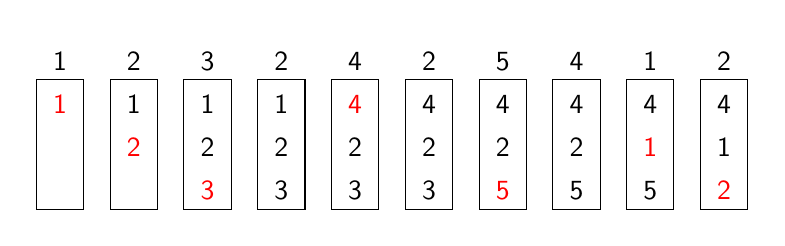
\begin{tikzpicture}[
    ampersand replacement=\&,
    every node/.style={
      align=center,
      text height=2ex,
      text width=1em
    },
    swapin/.list={
      (2,1),
      (3,2),
      (4,3),
      (2,5),
      (4,7),
      (3,9),
      (4,10)
    },
  ]
    \matrix (m) [
      matrix of nodes,
      nodes in empty cells,
      column sep=1em,
    ] {
      1 \& 2 \& 3 \& 2 \& 4 \& 2 \& 5 \& 4 \& 1 \& 2 \\
      1 \& 1 \& 1 \& 1 \& 4 \& 4 \& 4 \& 4 \& 4 \& 4 \\
        \& 2 \& 2 \& 2 \& 2 \& 2 \& 2 \& 2 \& 1 \& 1 \\
        \&   \& 3 \& 3 \& 3 \& 3 \& 5 \& 5 \& 5 \& 2 \\
    };
    \draw (m-2-1.north west) rectangle (m-4-1.south east);
    \draw (m-2-2.north west) rectangle (m-4-2.south east);
    \draw (m-2-3.north west) rectangle (m-4-3.south east);
    \draw (m-2-4.north west) rectangle (m-4-4.south east);
    \draw (m-2-5.north west) rectangle (m-4-5.south east);
    \draw (m-2-6.north west) rectangle (m-4-6.south east);
    \draw (m-2-7.north west) rectangle (m-4-7.south east);
    \draw (m-2-8.north west) rectangle (m-4-8.south east);
    \draw (m-2-9.north west) rectangle (m-4-9.south east);
    \draw (m-2-10.north west) rectangle (m-4-10.south east);
  \end{tikzpicture}

  \hspace{2em} 7 page faults.
}{
  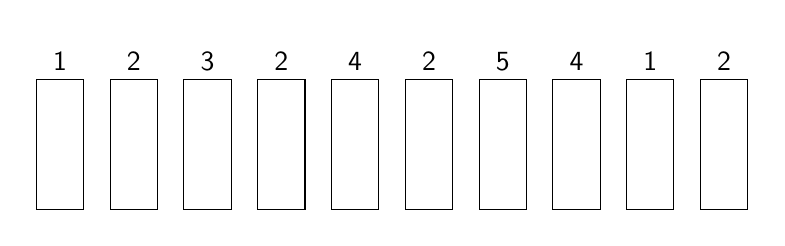
\begin{tikzpicture}[
    ampersand replacement=\&,
    every node/.style={
      align=center,
      text height=2ex,
      text width=1em
    },
  ]
    \matrix (m) [
      matrix of nodes,
      nodes in empty cells,
      column sep=1em,
    ] {
      1 \& 2 \& 3 \& 2 \& 4 \& 2 \& 5 \& 4 \& 1 \& 2 \\
        \&   \&   \&   \&   \&   \&   \&   \&   \&   \\
        \&   \&   \&   \&   \&   \&   \&   \&   \&   \\
        \&   \&   \&   \&   \&   \&   \&   \&   \&   \\
    };
    \draw (m-2-1.north west) rectangle (m-4-1.south east);
    \draw (m-2-2.north west) rectangle (m-4-2.south east);
    \draw (m-2-3.north west) rectangle (m-4-3.south east);
    \draw (m-2-4.north west) rectangle (m-4-4.south east);
    \draw (m-2-5.north west) rectangle (m-4-5.south east);
    \draw (m-2-6.north west) rectangle (m-4-6.south east);
    \draw (m-2-7.north west) rectangle (m-4-7.south east);
    \draw (m-2-8.north west) rectangle (m-4-8.south east);
    \draw (m-2-9.north west) rectangle (m-4-9.south east);
    \draw (m-2-10.north west) rectangle (m-4-10.south east);
  \end{tikzpicture}

  \hspace{2em} \_ page faults.
}

\vspace{21em}

\textbf{1b.} (10 points)
Now, use the optimal algorithm for page replacement.
All the other constraints are the same as the previous question.
For each access write all the pages in memory \textit{after the access} in the
boxes below.
State the number of page faults after all the accesses.

\vspace{1em}

\ifbool{solutions}{
  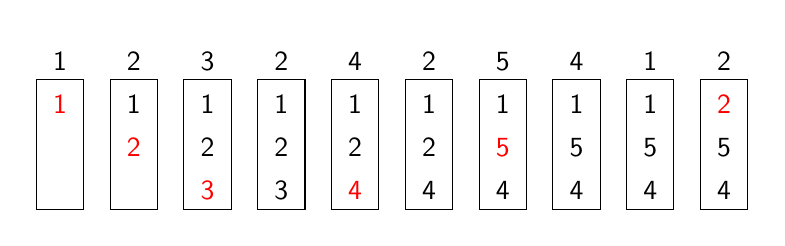
\begin{tikzpicture}[
    ampersand replacement=\&,
    every node/.style={
      align=center,
      text height=2ex,
      text width=1em
    },
    swapin/.list={
      (2,1),
      (3,2),
      (4,3),
      (4,5),
      (3,7),
      (2,10)
    },
  ]
    \matrix (m) [
      matrix of nodes,
      nodes in empty cells,
      column sep=1em,
    ] {
      1 \& 2 \& 3 \& 2 \& 4 \& 2 \& 5 \& 4 \& 1 \& 2 \\
      1 \& 1 \& 1 \& 1 \& 1 \& 1 \& 1 \& 1 \& 1 \& 2 \\
        \& 2 \& 2 \& 2 \& 2 \& 2 \& 5 \& 5 \& 5 \& 5 \\
        \&   \& 3 \& 3 \& 4 \& 4 \& 4 \& 4 \& 4 \& 4 \\
    };
    \draw (m-2-1.north west) rectangle (m-4-1.south east);
    \draw (m-2-2.north west) rectangle (m-4-2.south east);
    \draw (m-2-3.north west) rectangle (m-4-3.south east);
    \draw (m-2-4.north west) rectangle (m-4-4.south east);
    \draw (m-2-5.north west) rectangle (m-4-5.south east);
    \draw (m-2-6.north west) rectangle (m-4-6.south east);
    \draw (m-2-7.north west) rectangle (m-4-7.south east);
    \draw (m-2-8.north west) rectangle (m-4-8.south east);
    \draw (m-2-9.north west) rectangle (m-4-9.south east);
    \draw (m-2-10.north west) rectangle (m-4-10.south east);
  \end{tikzpicture}

  \hspace{2em} 6 page faults.
}{
  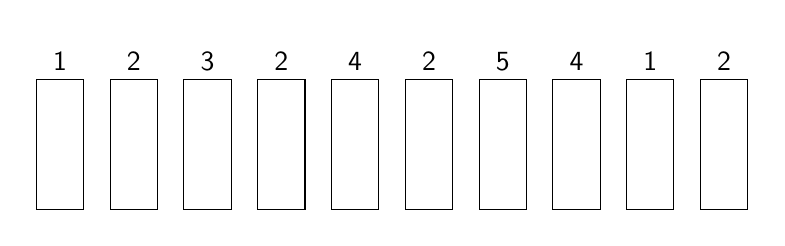
\begin{tikzpicture}[
    ampersand replacement=\&,
    every node/.style={
      align=center,
      text height=2ex,
      text width=1em
    },
  ]
    \matrix (m) [
      matrix of nodes,
      nodes in empty cells,
      column sep=1em,
    ] {
      1 \& 2 \& 3 \& 2 \& 4 \& 2 \& 5 \& 4 \& 1 \& 2 \\
        \&   \&   \&   \&   \&   \&   \&   \&   \&   \\
        \&   \&   \&   \&   \&   \&   \&   \&   \&   \\
        \&   \&   \&   \&   \&   \&   \&   \&   \&   \\
    };
    \draw (m-2-1.north west) rectangle (m-4-1.south east);
    \draw (m-2-2.north west) rectangle (m-4-2.south east);
    \draw (m-2-3.north west) rectangle (m-4-3.south east);
    \draw (m-2-4.north west) rectangle (m-4-4.south east);
    \draw (m-2-5.north west) rectangle (m-4-5.south east);
    \draw (m-2-6.north west) rectangle (m-4-6.south east);
    \draw (m-2-7.north west) rectangle (m-4-7.south east);
    \draw (m-2-8.north west) rectangle (m-4-8.south east);
    \draw (m-2-9.north west) rectangle (m-4-9.south east);
    \draw (m-2-10.north west) rectangle (m-4-10.south east);
  \end{tikzpicture}

  \hspace{2em} \_ page faults.
}

\newpage

\textbf{Question 2.} Threading (40 points total)

\vspace{1em}

Jon writes an... interesting server that allows remote clients to run the
\texttt{ls} command on it.
I don't know why Jon did it, but he did.
Maybe he was tired from running home to get his laptop.
For the code example, assume no errors occur and all system calls are
successful.
As a reminder, the file descriptor returned from \texttt{accept} can be used
in subsequent \texttt{read} and \texttt{write} system calls.
Consider the following code:

\vspace{1em}

\begin{lstlisting}
void* run(void* arg) {
  int fd = (int) arg;
  sleep(5);
  pid_t pid = fork();
  if (pid == 0) {
    dup2(fd, 1);
    execlp("ls", "ls", NULL);
  }
  return NULL;
}

int main() {
  int socket_fd;
  /* Setup the socket (calls socket, bind, listen) */
  while (true) {
    int fd = accept(socket_fd, NULL, NULL);
    pthread_t thread;
    pthread_create(&thread, NULL, run, (void*) fd);
    pthread_detach(thread);
  }
  return 0;
}
\end{lstlisting}

\vspace{1em}

Again, assume no errors occur.
There's some weird casting, but at the end of the day, all we're doing is
passing \texttt{fd} to a thread.

\vspace{1em}

\textbf{2a.} (2 points)
Assume 4 clients connect and each one makes it to the call to \texttt{sleep(5)}
and none return from \texttt{sleep} yet.
How many threads are there \textit{in total} and what are they executing in the
code?

\vspace{3em}

\textbf{2b.} (10 points)
Now, all threads return from \texttt{sleep} and complete.
What gets sent back over the socket, and why?

\newpage

\ 

\vspace{7em}

\textbf{2c.} (3 points)
How many processes did we create (excluding the original running process)?

\vspace{3em}

\textbf{2d.} (10 points)
What did we forget to do with the newly created porcesses?
Why is this especially an issue in this case where our server runs for a very
long time and may end up serving thousands of requests?

\vspace{16em}

\textbf{2e.} (5 points)
What would happen if we did not \texttt{fork} and instead always executed
\texttt{dup2} followed by \texttt{execlp} directly after the \texttt{sleep} in
every thread?

\vspace{11em}

\textbf{2f.} (10 points)
What would be the issue if we removed \texttt{pthread\_detach}?

\newpage

\textbf{Question 3.} Locks (20 points total)

\vspace{1em}

You were given a \texttt{transfer} function to safely transfer funds between two
accounts.
You decided to refactor it such that there's a separate function for deducting
(removing) funds from an account.
Assume that multiple threads can call \texttt{transfer} simultaneously
using different accounts.
Consider your initial implementation:

\vspace{1em}

\begin{lstlisting}
struct account {
  pthread_mutex_t mutex;
  char* name;
  int amount;
}

void transfer(struct account* from, struct account* to, int amount) {
  if (from == to) return;
  pthread_mutex_lock(&to->mutex);
  to->amount += deduct(from, amount);
  pthread_mutex_unlock(&to->mutex);
}

/* Returns the amount of money deducted from an account.
   An account cannot go negative. */
int deduct(struct account* account, int amount) {
  pthread_mutex_lock(&account->mutex);
  if (account->amount >= amount) {
    account->amount -= amount;
  }
  else {
    amount = 0;
  }
  pthread_mutex_unlock(&account->mutex);
  return amount;
}
\end{lstlisting}

\vspace{1em}

Again, assume no errors occur.

\vspace{1em}

\textbf{3a.} (5 points)
Does this code have any data races? Come up with an example of a data race if
it does, or justify why it does not.

\newpage

\textbf{3b.} (5 points)
Does this code have any deadlocks? Come up with an example of a deadlock if
it does, or justify why it does not.

\vspace{20em}

\textbf{3c.} (10 points)
Given the issue(s) you found in 3a and 3b, explain how you would fix the code
to prevent those issues.
You may not significantly refactor the given code.
That means \texttt{transfer} must add to the \texttt{to} account and call
\texttt{deduct}.
Also, \texttt{deduct} must safely decrement the account only if it won't have
an negative amount, otherwise it must be 0.
\texttt{deduct} always returns the amount deducted.
You may write replacement functions, or explain yourself clearly.

\newpage

\textbf{Question 4.} Locking (20 points total)

\vspace{1em}

You're given 4 threads (that get properly created and run) and you want to
ensure ordering between them.
You decide to use semaphores to accomplish your task.
Recall that semaphores, after initialization, use
\texttt{sem\_post(sem\_t* sem)} to increment the value and
\texttt{sem\_wait(sem\_t* sem)} to decrement the value (waiting until the value
is greater than 0).
Assume no errors occur, so you never need to check return values.
Consider the following code:

\begin{lstlisting}
/* Global variables */ sem_t sem1; sem_t sem2; sem_t sem3;

void initialize() {
  sem_init(&sem1, 0, _);
  sem_init(&sem2, 0, _);
  sem_init(&sem3, 0, _);
}
void* thread1(void*) {
  f1();


  f2();


}
void* thread2(void*) {


  f3(); /* only runs after f1 completes */


}
void* thread3(void*) {


  f4() /* only runs after f1 completes */;


}
void* thread4(void*) {


  f5(); /* only runs after f2 completes */


  f6(); /* only runs after f3 and f4 complete */
}
\end{lstlisting}

\newpage

\textbf{4a.} (10 points) Fill in the initial values for each semaphore and
insert \texttt{sem\_post} and \texttt{sem\_wait} calls in a way that ensures
the ordering in the comments.
You cannot change the ordering of the \texttt{f()} calls, and they always
execute in the order written.
Write your answers on the previous page.

\vspace{1em}

\textbf{4b.} (10 points) For each function state which functions \textit{could}
run in parallel with it (not including itself).
Write ``none'' if it can only run by itself.

\vspace{1em}

\texttt{f1}:

\vspace{3em}

\texttt{f2}:

\vspace{3em}

\texttt{f3}:

\vspace{3em}

\texttt{f4}:

\vspace{3em}

\texttt{f5}:

\vspace{3em}

\texttt{f6}:

\newpage

\textbf{Question 5.} Memory Allocation (10 points total)

\vspace{1em}

You decide to use a buddy allocator to handle a bunch of fixed-sized allocations
(it was too early and you slept through slab allocators).
Your allocator needs to be able to handle 8 allocations of 10 bytes each.

\vspace{1em}

\textbf{5a.} (5 points)
How big of a memory block does your buddy allocator need at minimum to be able
to handle every allocation?
Justify your answer.

\vspace{16em}

\textbf{5b.} (5 points)
How many bytes are lost due to fragmentation and what type of fragmentation is
this?
Justify your answer.

\newpage

\textbf{Question 6.} Disks (10 points total)

\vspace{1em}

Inspired by the course, and your data hoarding, you decide you'd like to build
yourself a RAID.
You buy yourself 8 hard drives that are 4 TB each.

\vspace{1em}

\textbf{6a.} (2 points)
What RAID configuration would you use if you really really care about your data?
Justify your answer.

\vspace{11em}

\textbf{6b.} (3 points)
What RAID configuration would you use if you care about your data but want more
than 4 TB of total capacity?
Justify your answer.

\vspace{16em}

\textbf{6c.} (5 points)
What RAID configuration would you use if you only care about performance?
Justify your answer.
Also state how much faster your read and write performance would be compared to
a single disk.

\newpage

\textbf{Question 7.} Filesystems (10 points total)

\vspace{1em}

You'll be using your knowledge of filesystems to explain the difference between
\texttt{ln} and \texttt{cp} in terms of inodes and blocks.
Assume you have a file called \texttt{my-file.txt} that contains 2290 bytes.
The block size of the filesystem is 4096 bytes, so it fits on a single block.
As a hint, I ran the \texttt{ln} and \texttt{cp} commands and you'll find the
output of \texttt{ls} after the commands below:

\vspace{1em}

\begin{lstlisting}
> ln my-file.txt ln-file.txt
> cp my-file.txt cp-file.txt
> ls
inode   size   name
  101   2290   my-file.txt
  102   2290   cp-file.txt
  101   2290   ln-file.txt
\end{lstlisting}

\vspace{1em}

\textbf{7a.} (5 points)
Explain what happens on the filesystem when you run the \texttt{ln} command.
Start your explaination with the new directory entry for \texttt{ln-file.txt}.

\vspace{16em}

\textbf{7b.} (5 points)
Explain what happens on the filesystem when you run the \texttt{cp} command.
Start your explaination with the new directory entry for \texttt{cp-file.txt}.

\newpage

\textbf{Question 8.} Virtual Machines (10 points total)

\vspace{1em}

You have a single server that hosts a web server, database, and streams video.
Over time, as your server gets used more, you find that it's now overloaded.
You decide to buy another server.
You could move one of the three applications to the new server, and hope that
it's balanced.
Given you've taken this course, you think using virtual machines would be a good
idea (assume containers do not exist).

\vspace{1em}

\textbf{8a.} (5 points)
How would your organize your applications into virtual machines?
Explain how many virtual machines you would make and what would go on them.

\vspace{21em}

\textbf{8b.} (5 points)
What would be the benefits of using your virtual machines in the event your
one of the two servers is now overloaded?

\afterpage{\null\newpage}

\end{document}
